% !TeX spellcheck=en_GB
\section{Approximation Algorithms in General}
An approximation algorithm is an algorithm which returns near optimal solutions. Approximation algorithms has bounds on how \textit{far} away the solution can atmost be from the optimal solution. We say that the approximation ratio $p(n)$ denotes the bound of an approximation algorithm. That is if $C*$ is the optimal solutions and $C$ is the solution by the approximation algorithm, then $max(C*/C,C/C*) <= p(n)$. For example, if the approximation ratio is 2 then the algorithm is called a $2-Opt$ algorithm and the result is guaranteed to be at most twice as big as the optimal solution for minimization problems and at least half as much as the optimal solution for maximization problem.

The concept of Polynomial Time Approximation Scheme (PTAS) denotes $(1+\epsilon)$-approximation schemes which have polynomial running times in the size of the input but may be exponential in $1/\epsilon$. This implies that PTAS gets exponentially harder the closer the approximation bound is to optimal. The Fully Polynomial Time Approximation Scheme (FPTAS) on the other hand are both polynomial in the input size and $1/\epsilon$. 

In comparison, heuristics often do not have proven bounds on either running time or optimality ratio, but could in general give better results than approximation algorithms. In practise heuristics are often preferred over the more theoretically correct approximation algorithms simply because the worst case scenarios of the heuristics seldom happen.

\section{Vertex Cover}
The vertex cover problem is the problem of, given an undirected graph $G(V,E)$ to find a subset $C$ of $V$ such that every edge has at least one endpoint in $C$. The problem is NP-hard and can be generalized to give each vertex a cost, in which case the problem is called the weighted vertex cover. The optimization version of vertex cover is to find a cover of minimum size or minimum weight.

\subsection{Maximal Matching Approximation Algorithm}
A matching in a graph $G$ is a subset of edges in a graph which has no vertices in common. A matching can be maximal in which case it is not possible to add any edge to the subset without breaking the matching invariant. A maximum matching is a maximal matching which also has the largest size for the given graph. Note that there can still be multiple maximum matchings in a graph. 

Any maximal matching of a graph $G$ can be used to find a vertex cover over the same graph, by adding both endpoints of the edges in the matching. If there exists an edge which is not connected to any of the endpoints in the matching, then it has to be adjacent to two vertices not in the matching. In that case the edge could be added to the matching without violating the invariant and therefore the matching was not maximal to begin with. The idea of just using maximal matchings instead of maximum matchings is that maximum matchings contains more edges and therefore spans more vertices than a non-maximum but maximal matching. Since we want to minimize the size of the vertex cover just maximal matchings are preferred.

\begin{figure}[H]
    \centering
    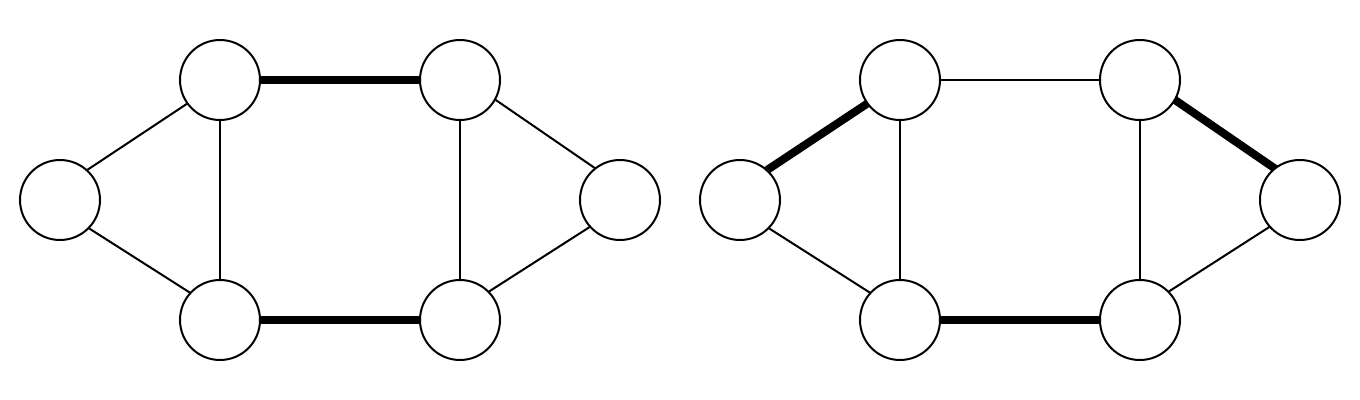
\includegraphics[width=\textwidth]{matchings}
    \caption{A maximal matching and a maximum matching of a graph with 6 vertices.}
\end{figure}

Using maximal matchings gives a 2-approximation algorithm for the vertex cover problem. This can easily be proven by looking at the size of the optimal cover $|C*|$ and the size of a maximal matching $|M|$ then $|M| < |C*|$ since every edge in the matching needs to be covered in $C*$. The size of the vertex cover based on the matching has size $|C|=2|M|$ and therefore we get that $|C| <= 2|C*|$. We can also show that the approximation ratio is tight, by constructing a bipartite graph with equally sized $A$ and $B$ vertex sets, where every element in $A$ is connected to every element in $B$. Here the approximation algorithm using maximal matchings will contain all vertices but the minimum vertex cover is achieved with only the vertices of either $A$ or $B$, hence only half the number of vertices.

\subsection{LP Approximation}
Integer Linear programming can be used as a basis for a 2-approximation algorithm for the weighted vertex cover. By solving the LP relaxation of the ILP and adding every vertex with value $1/2$ a vertex cover of atmost 2 times the optimal is created. The result is a vertex cover since there exists constraint on each vertex in the following form: $x_i + x_j \ge 1 \text{for every edge } (i,j) \in E$. Therefore if a variable $x_i$ of vertex $i$ has value below $1/2$ every edge with one endpoint in $i$ must be connected to another vertex with a variable with a value higher than $1/2$ and therefore covered by the approximation algorithm.

To prove that the algorithm is a 2-approximation we define $S*$ as the optimum vertex cover and $S$ the vertex cover achieved by the algorithm. By summing over the weights of the optimal values of the linear program and using the fact that every $x*_i \ge 1/2$ for all $i$ in S we can show that $w(S)$ is at most twice of $w(S*)$ by following equation: $\sum_{i \in S} w_i x*_i \ge 1/2 \sum_{i \in S} w_i = 1/2 w(S)$.

Another LP based approximation algorithm is the pricing method. The variables of the dual LP can be seen as describing the price each edge pays to be part of the cover. The objective is to maximize the profit from edges as much as possible. The price an edge can pay can be at most the weight of the vertices it is connected to. A vertex $i$ is said to be tight if its dual constraint has no slack, that is we cannot increase the price an edge incident to $i$ anymore without violating the constraints. This creates the base for the pricing approximation algorithm. $Y_e$ is set to 0 for every edge. Then while there exists an edge $(i,j)$ where neither vertex is tight increase the price edge $e$ pays until either $i$ or $j$ (or both) becomes tight. The vertex cover is then created from the tight vertices.

\begin{figure}[H]
    \centering
    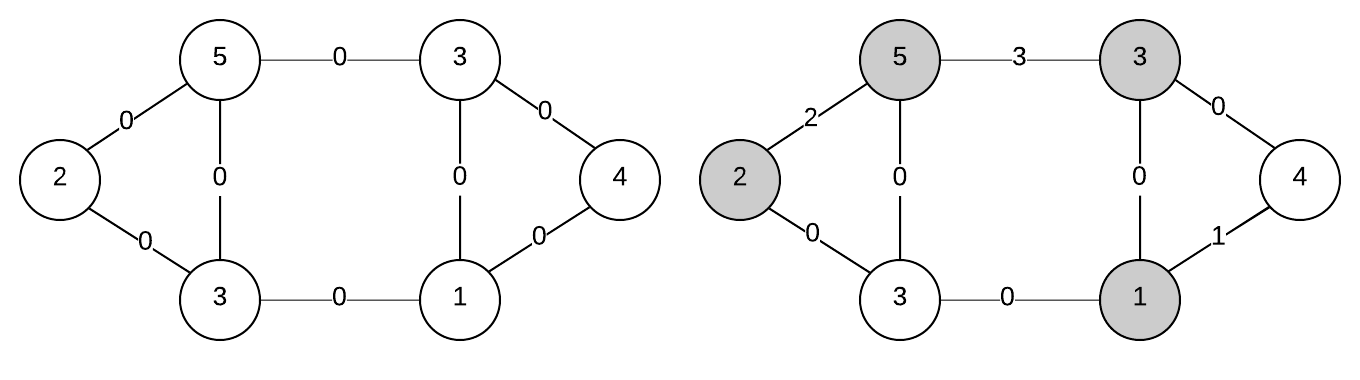
\includegraphics[width=\textwidth]{pricing}
    \caption{The number in each node is the weight of the vertex and the numbers on the edges is the paid price of that edge. The colored vertices are tight.}
\end{figure}

\newpar The pricing algorithm is polynomial since at least one vertex is added each iteration of the while loop and the result is a vertex cover since for every edge $(i,j)$ either vertices $i$ or $j$ or both are tight and therefore in the cover. 

\section{Metric Traveling Salesman Problem}
Some approximation algorithms only work for specific instances of certain problems such as the metric TSP where the graph is complete and the triangulation equality is satisfied. 

A 2-approximation algorithm for the metric TSP is to create a minimum spanning tree $T$ of $G$ and then to walk around $T$, taking short-cut to next vertex in a depth first search manner to avoid paying the cost of each edge twice. The result of this is clearly a Hamiltonian Tour $W$ which is also a solution to the TSP. The result can shown to be 2-Opt, by the following proof. Let $W*$ be the optimal solution, if we remove any edge $e$ from $W*$ we get a tree and therefore $|W*| \ge |W*| - |e| \ge |T|$. The walk around a spanning tree is twice the size of the spanning tree and therefore we get $W \le 2|T| \le 2|W*|$ which concludes the proof.
 
\newpar LAV EKSEMPSEL TODO TODO TODO TODO TODO TODO

\newpar An even better bound can be achieved by combining the concept of matchings and minimum spanning trees. First a minimum spanning tree is generated. In a tree there can only be an even number of vertices with uneven degree and therefore a minimum weight matching is created between vertices with odd degree. The matchings are added to the MST (allowing multi edges) and a walk around the graph is constructed without reusing the same edge twice. If multi edges are used they are removed and short-cuts are taken to make the walk a tour. This approach gives a $2/3$-approximation. The proof of the bound is omitted from these lecture notes.

\newpar LAV EKSEMPSEL TODO TODO TODO TODO TODO TODO

\section{Knapsack}
Due to time and space constraints only the $1/\epsilon$-approximation algorithm is explained in these lecture notes. In the knapsack problem, $n$ items with a weight and a profit must be packed to optimize profit while adhering to a maximum capacity/volume $V$. This problem is NP-hard but there exists a pseudo polynomial algorithm, that is it is polynomial in the size of $n$ but the running time is also polynomial in the size of $P$(the largest profit of an item) which can be very large and therefore make the problem difficult even for small $n$. This pseudo polynomial algorithm has been left out of the notes. The approximation algorithm is based on the idea of downscaling $P$ to make the algorithm faster while only creating small errors. The algorithm chooses a scaling factor $K$ based on the wanted ratio to optimality $K=\epsilon P/n$, then for each object $p*_i = \lfloor p_i/K \rfloor$.

For example if we have the following profits $\{ 200, 100, 95 \}$ where the first element of the tuples is the profit and the second is the volume. If we want a 1/2-approximation scheme we calculate $K=\frac{1/2*200}{4} = 25$. Tthe profits are then scaled to $\{ 8, 4, 3 \}$. Note here that we floor $95/25=3.8$ which means we loose some precision from the original problem. The two other profits keep their ratio.

\newpar The running time is $\mathcal{O}(n^2 floor(P/K) \equiv \mathcal{O}(n^2 floor(n/\epsilon)$ and is therefore an example of an algorithm which is both polynomial in $n$ and in $1/\epsilon$ and hence is an FPTAS. We can furthermore see that the solution obtained is at most $1+\epsilon$-Opt by the following proof: Let $O$ be the optimal solution, $S$ be the solution from the approximation algorithm, $p(x)$ be the profit of the solution $x$ given the unscaled profits and $p*(x)$ given the scaled profits. Since there are $n$ objects and each objects profit is at most scaled by K we get $p(O) - K*p*(O) \le nK$. Then we have $p(S) \ge Kp*(O) \ge p(O)-n K$. By using the definition of K $n K$ becomes $n (\epsilon P/n)$ and we get $p(O) - \epsilon P \ge (1-\epsilon) p(O)$. This shows us that the scaling algorithm is a $(1+\epsilon)$-approximation algorithm to the knapsack problem.
